\chapter{三选一任务}

\section{设计目的}

任务三 频率计仿真和综合

1、按下列功能要求,使用 verilog 语言编写 RTL 代码及对应测试代码

用状态机设计一个自动转换量程的频率计的控制部分,用case语句描述。

2、仿真调试完成后,按下列要求综合,最后版图设计

按下列要求完成约束文件的编写:

\begin{itemize}
    \item 建立名为 \texttt{my\_clk} 的250Mhz的时钟;
    \item 设置时钟漂移为0.25ns;
    \item 时钟寄存器不与时钟网络连接;
    \item 设置除时钟外输入端口的表达式,类似宏定义;
    \item 设置除时钟外输入端口最大延时为1ns;
    \item 设置输出端口延时为3ns。
\end{itemize}

综合后生成timing.rpt文件,检查确保slack>0,生成.sdf文件,用于后仿真,

其中:
clk: 为同步时钟信号;
Clr: 为异步复位信号。

\section{设计思路}

目的是实现频率计的控制模块,使用状态机管理自动量程转换逻辑。通过时钟信号和异步清零信号驱动状态切换,当清零信号触发时,状态初始化为STATE\_C。状态转换根据计数溢出(Cntover)或计数偏低(Cntlow)条件进行。在不同状态下,模块设置特定的量程(range)、频率选择信号(std\_f\_sel),并根据需要控制复位信号(reset)。组合逻辑部分确保每次状态切换时输出信号与相应状态匹配,并通过case语句管理六种状态间的跳转,确保量程自动切换的逻辑满足频率计的控制需求。

% project 构造参考例程

\section{设计步骤}

\subsection{RTL 代码编写}

% show code

\begin{minted}[
    frame=lines,
    framesep=2mm,
    baselinestretch=1.2,
    bgcolor=lightgray!20,
    fontsize=\small,
    linenos
  ]{verilog}
  `timescale 1ns/1ps

  module frequency_counter_control(
      input wire Clk,
      input wire Clear,
      input wire Cntover,
      input wire Cntlow,
      output reg reset,
      output reg [1:0] std_f_sel,
      output reg [2:0] range
  );
      reg [2:0] state, next_state;
  
      // 定义状态参数
      localparam STATE_A = 3'b000, // 100K stateA
                 STATE_B = 3'b001, // 100K stateB
                 STATE_C = 3'b010, // 10K stateC
                 STATE_D = 3'b011, // 10K stateD
                 STATE_E = 3'b100, // 1K stateE
                 STATE_F = 3'b101; // 1K stateF
  
      // 时序逻辑:状态切换
      always @(posedge Clk or posedge Clear) begin
          if (Clear)
              state <= STATE_C;  // 初始化为 STATE_C
          else
              state <= next_state;
      end
  
      // 组合逻辑:状态转移和输出控制
      always @(*) begin
          // 默认值初始化,减少冗余赋值
          range = 3'b010;
          std_f_sel = 2'b01;
          reset = 1;
          next_state = state;  // 默认保持当前状态
  
          case (state)
              STATE_A: begin
                  range = 3'b000;
                  std_f_sel = 2'b00;
                  next_state = STATE_B;
              end
  
              STATE_B: begin
                  range = 3'b000;
                  std_f_sel = 2'b00;
                  reset = 0;
                  if (Cntlow)
                      next_state = STATE_C;
              end
  
              STATE_C: begin
                  range = 3'b010;
                  std_f_sel = 2'b01;
                  next_state = STATE_D;
              end
  
              STATE_D: begin
                  range = 3'b010;
                  std_f_sel = 2'b01;
                  reset = 0;
                  if (Cntover)
                      next_state = STATE_A;
                  else if (Cntlow)
                      next_state = STATE_E;
              end
  
              STATE_E: begin
                  range = 3'b100;
                  std_f_sel = 2'b11;
                  next_state = STATE_F;
              end
  
              STATE_F: begin
                  range = 3'b100;
                  std_f_sel = 2'b11;
                  reset = 0;
                  if (Cntover)
                      next_state = STATE_C;
              end
  
              default: begin
                  next_state = STATE_C;
              end
          endcase
      end
  endmodule
\end{minted}  

\subsection{测试代码编写与仿真调试}

通过搭建简单的testbench检验设计代码的正确性,tb\_frequency\_counter\_control.v文件为 verilog 测试平台代码。

% show code

\begin{figure}[H]
    \centering
    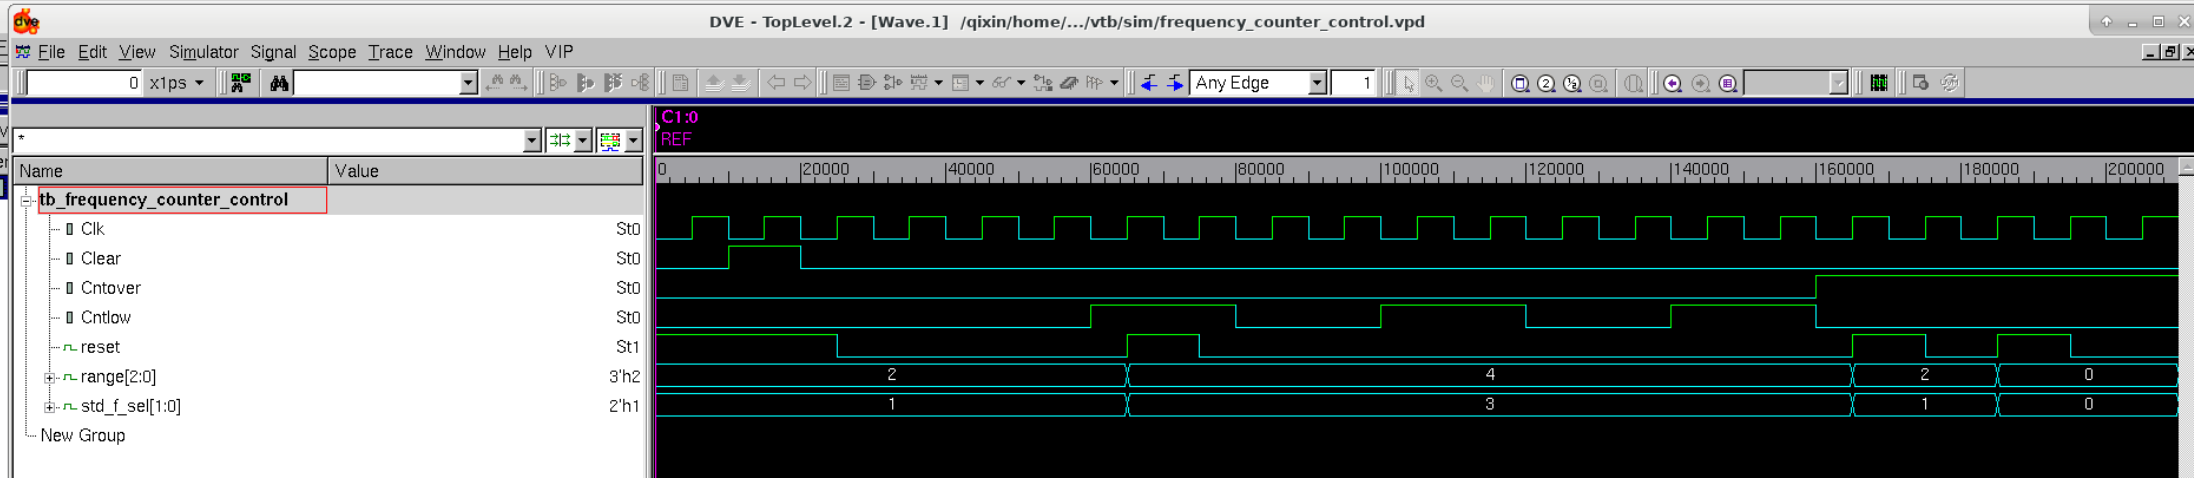
\includegraphics[width=0.8\textwidth]{images/final-task03-01.png}
    \caption{图1 仿真波形}
\end{figure}

进入仿真目录 verify/vtb/sim ,执行 make 命令,使用VCS数字逻辑仿真工具编译RTL和测试平台并进行仿真

\subsection{约束文件编写}

用 DC 工具进行编译和综合。

完成 frequency\_counter\_control.sdc 的编写后,进行综合。

% show code

\begin{minted}[
    frame=lines,
    framesep=2mm,
    baselinestretch=1.2,
    bgcolor=lightgray!20,
    fontsize=\small,
    linenos
  ]{text}
  create_clock -name my_clk -period 4.0 [get_ports Clk]

  set_clock_uncertainty 0.25 [get_clocks my_clk]
  
  set_dont_touch_network [get_clocks my_clk]
  
  set_input_delay -max 1.0 [get_ports {Clear reset Cntover Cntlow}]
  
  set_input_delay -max 1.0 [get_ports {Clear reset Cntover Cntlow}] -clock my_clk
  
  set_output_delay -max 3.0 [get_ports {range std_f_sel}] -clock my_clk
  
  set_output_delay -min 0.0 -max 3.0 [get_ports {range std_f_sel}] -clock my_clk
  
  set_dont_touch [get_ports {Clear reset Cntover Cntlow}]
\end{minted}

以上约束文件的作用分别是:

1、创建一个名为 my\_clk 的时钟信号,并指定其周期为 4.0 ns。时钟频率为 250MHz。

2、为 my\_clk 时钟设置 不确定性(uncertainty)为 0.25 ns。

3、禁止工具对 my\_clk 的时钟网络进行任何优化。

4、设置输入端口 Clear reset Cntover Cntlow 的最大输入延迟为 1.0 ns。

5、将输入延迟约束与时钟 my\_clk 关联起来

6、设置输出端口 range std\_f\_sel 的最大输出延迟为 3.0 ns,与 my\_clk 时钟同步。

7、进一步细化输出延迟,指定最小延迟为 0.0 ns,最大延迟为 3.0 ns。

8、禁止工具对这些输入端口进行优化。


1、	进入到dc路径下,启动dc,键入: \texttt{dc\_shell}

2、	在dc\_shell命令框下输入命令: \texttt{source run\_dc.tcl}
注:run\_dc.tcl 是一个tcl脚本,主要实现了Design Compiler的详细步骤。

3、	在命令栏输入 \texttt{report\_timing}

\begin{figure}[H]
    \centering
    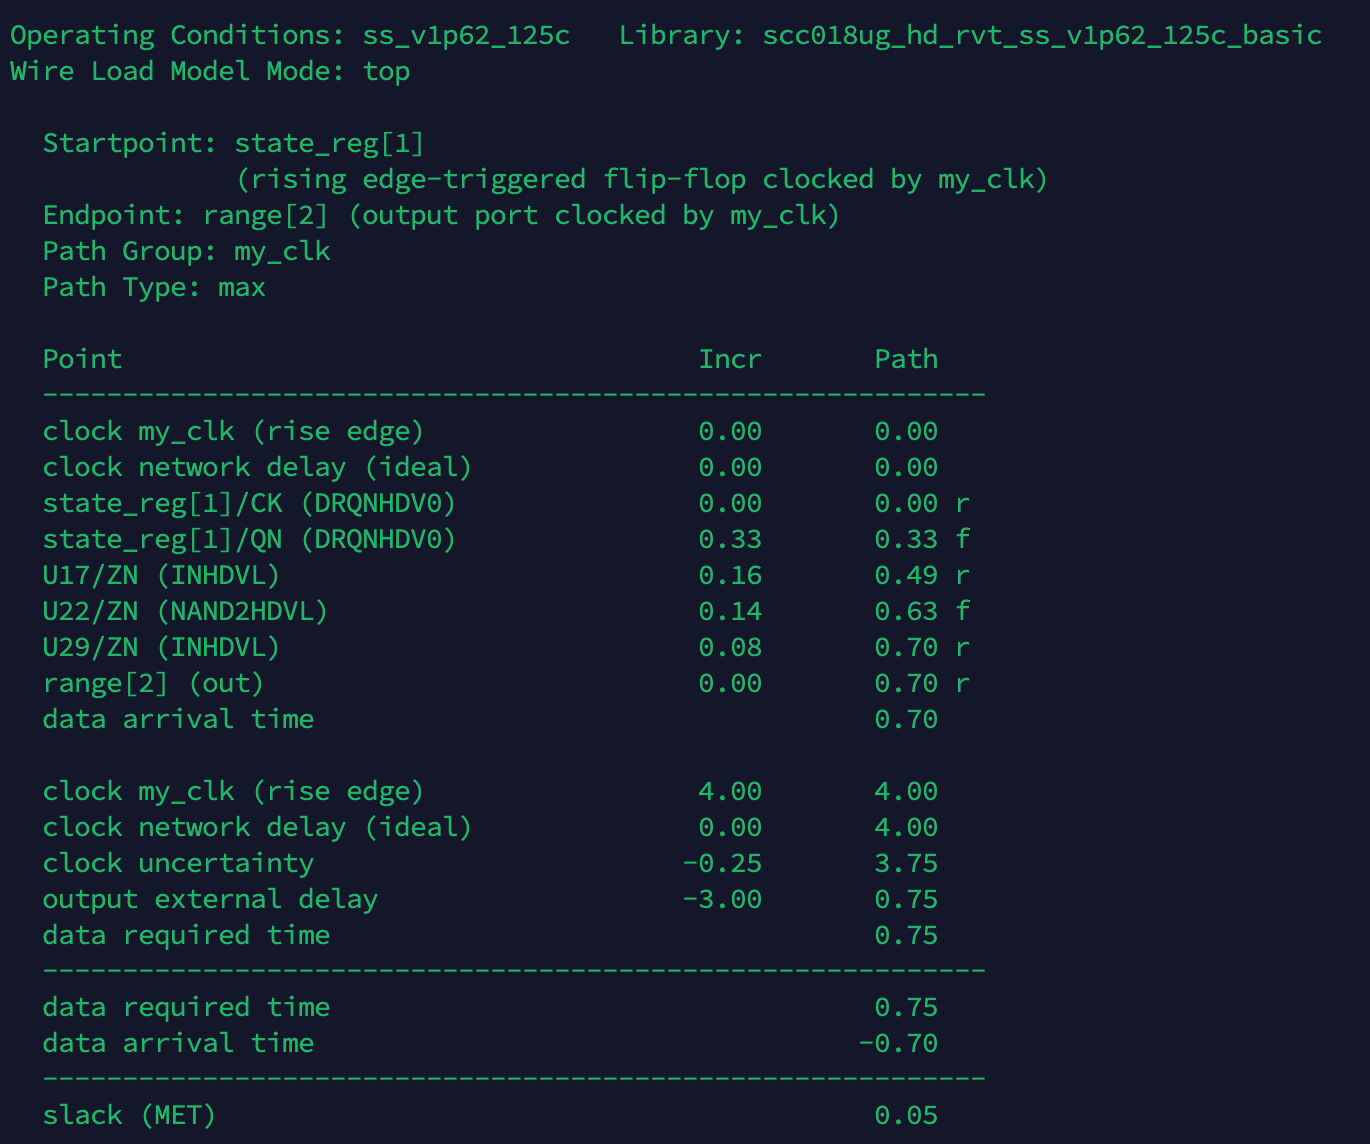
\includegraphics[width=0.8\textwidth]{images/final-task03-02.png}
    \caption{图2 综合结果}
\end{figure}

如图所示 slack 值为正数,则表明设计满足时序要求

\subsection{Formal}

1、验证综合前后的网表逻辑等价性检查。
2、验证综合后的网表与绕线后的网表逻辑等价性检查。

分别运行 \texttt{run\_G2G.tcl} 和 \texttt{run\_R2G.tcl} 脚本,进行Formal验证。如图所示通过:

\begin{figure}[H]
    \centering
    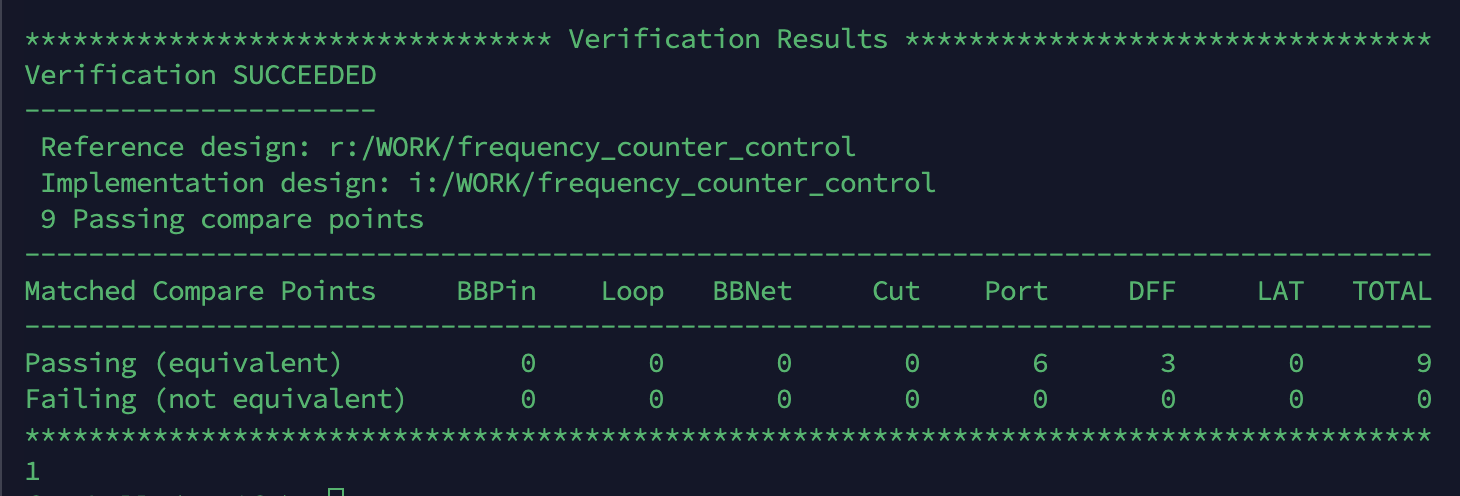
\includegraphics[width=0.8\textwidth]{images/final-task03-11.png}
    \caption{G2G}
\end{figure}

\begin{figure}[H]
    \centering
    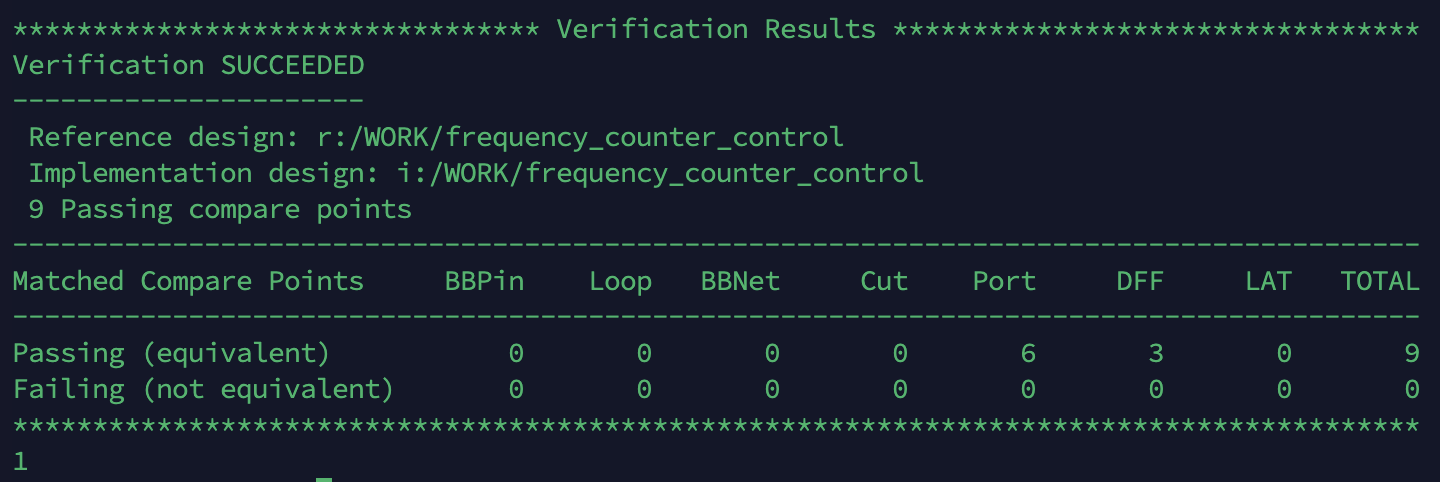
\includegraphics[width=0.8\textwidth]{images/final-task03-12.png}
    \caption{R2G}
\end{figure}

\subsection{版图设计}

使用TCL脚本使用innovus工具进行布局布线。

首先将 syn/dc/frequency\_counter\_control.v 到 pr/ 目录下。

编辑 run\_innovus.tcl 和 viewDefinition.tcl 文件,随后运行 \texttt{innovus -files run\_innovus.tcl}。

运行 \texttt{check\_timing -verbose > check.rpt},然后打开 check.rpt,查看时序报告。

\begin{figure}[H]
    \centering
    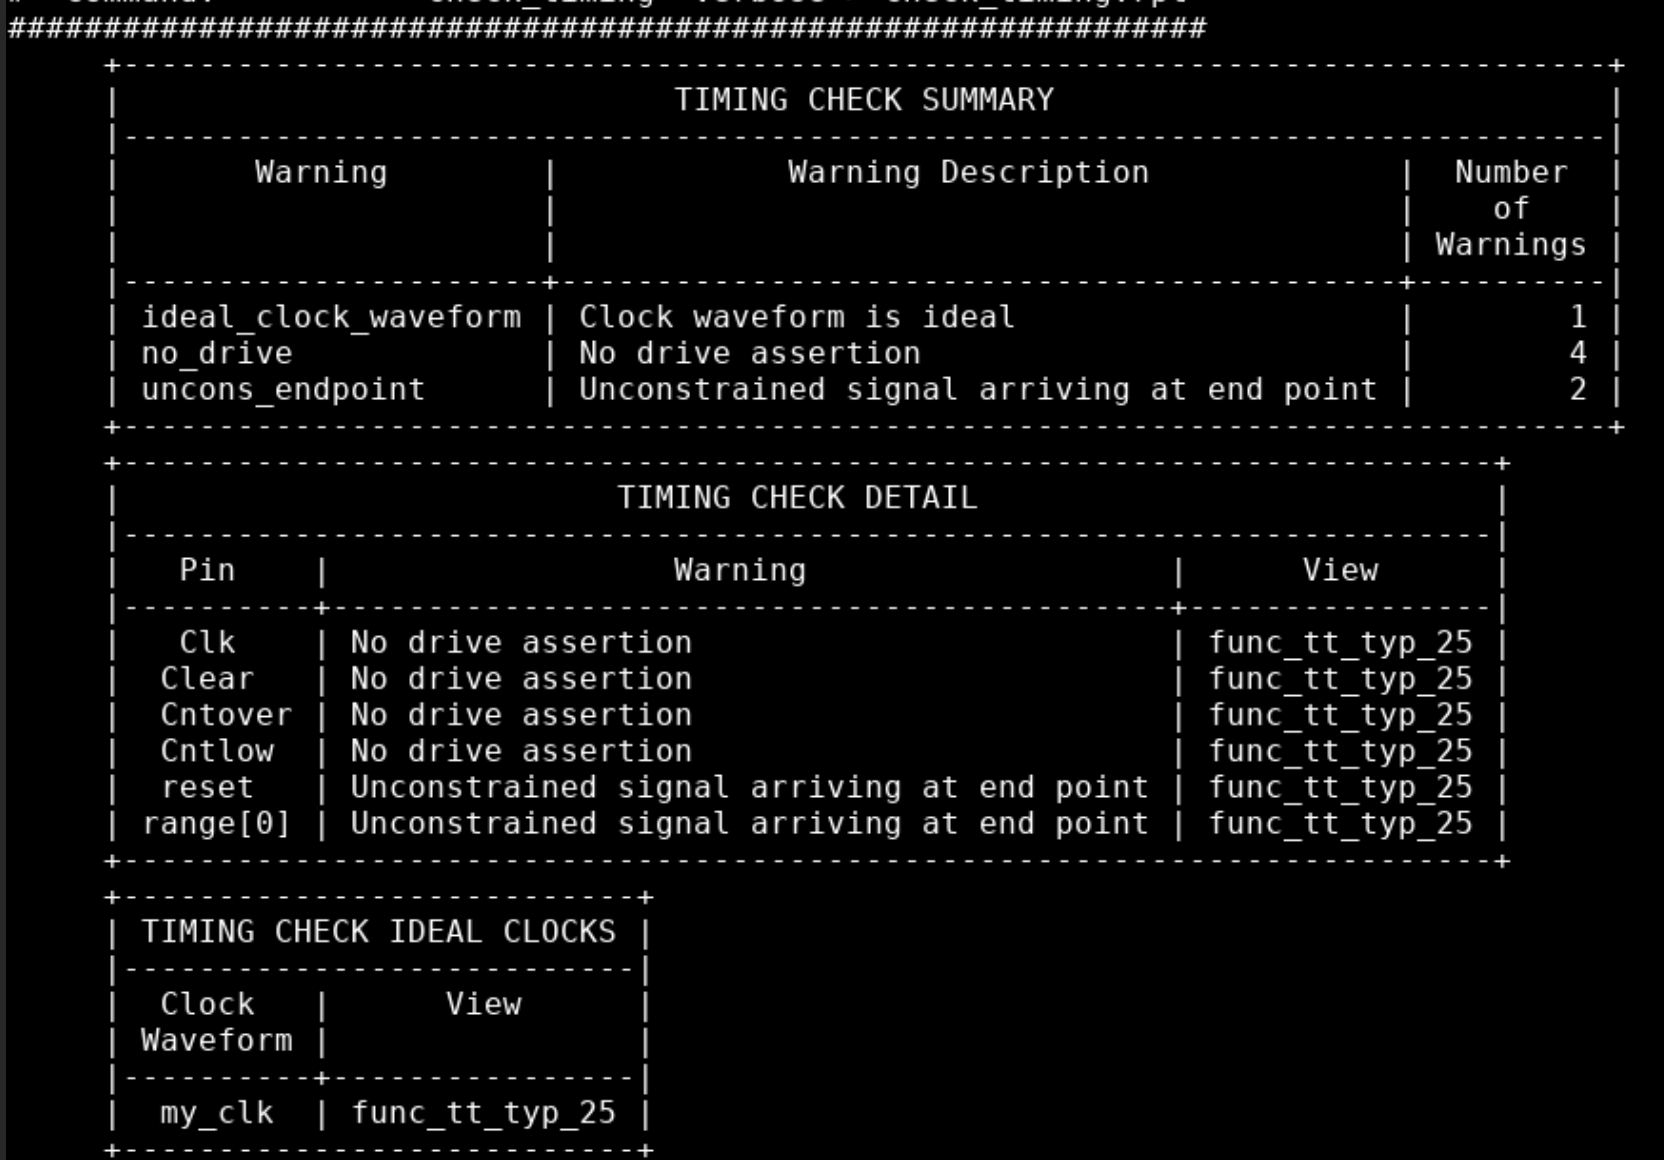
\includegraphics[width=0.8\textwidth]{images/final-task03-03.png}
    \caption{图4 时序报告}
\end{figure}

运行 \texttt{timeDesign -prePlace},  报出 timing 情况

\begin{figure}[H]
    \centering
    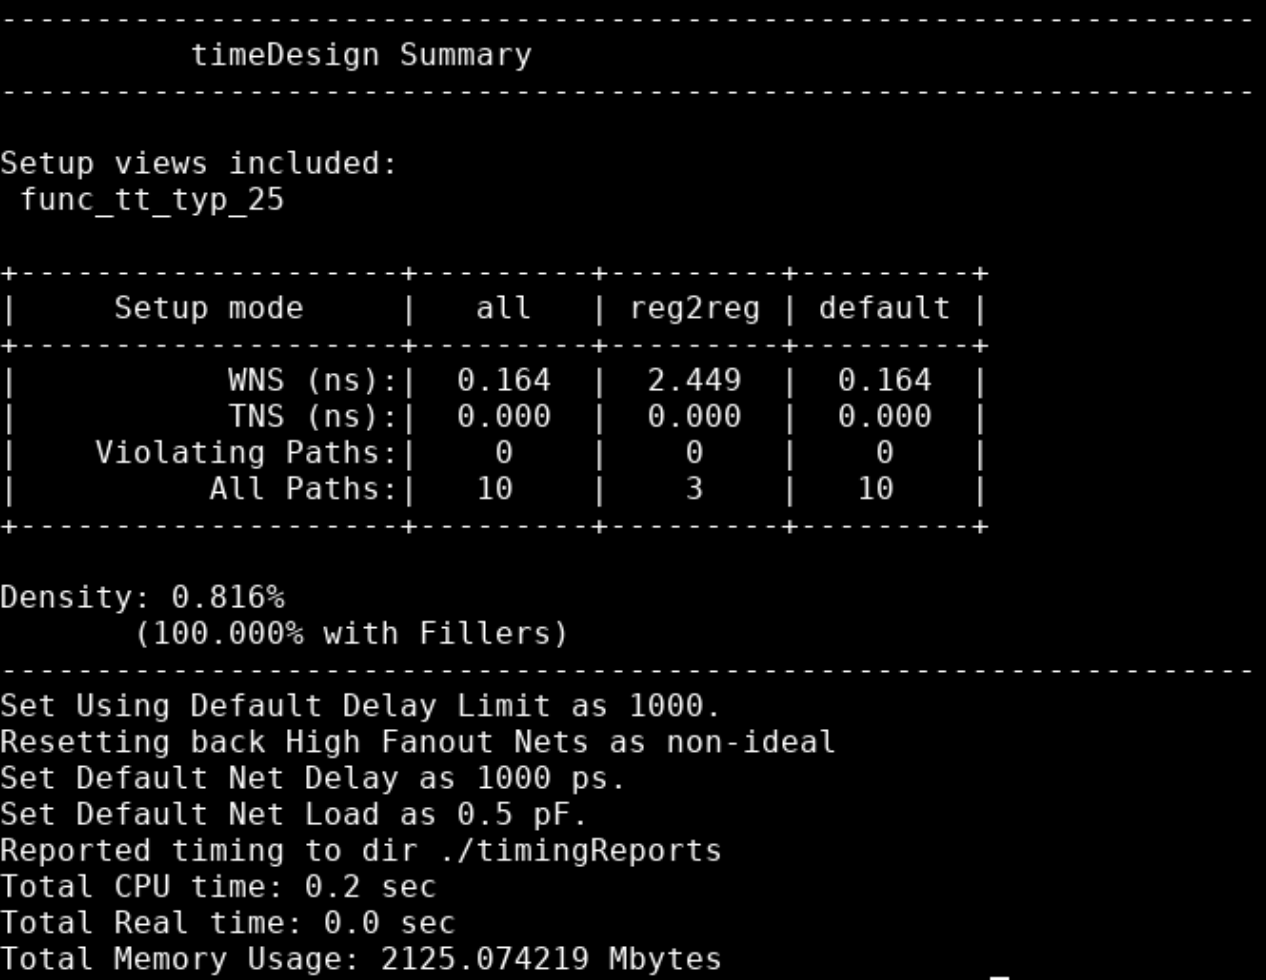
\includegraphics[width=0.8\textwidth]{images/final-task03-04.png}
    \caption{图5 时序报告}
\end{figure}

完成布局规划,通过继续运行 \texttt{run\_innovus\_step\_1\_floorplan.tcl} 进行布局布线。

1) 制定芯片面积

2) 完成 IO pin 分配

\begin{figure}[H]
    \centering
    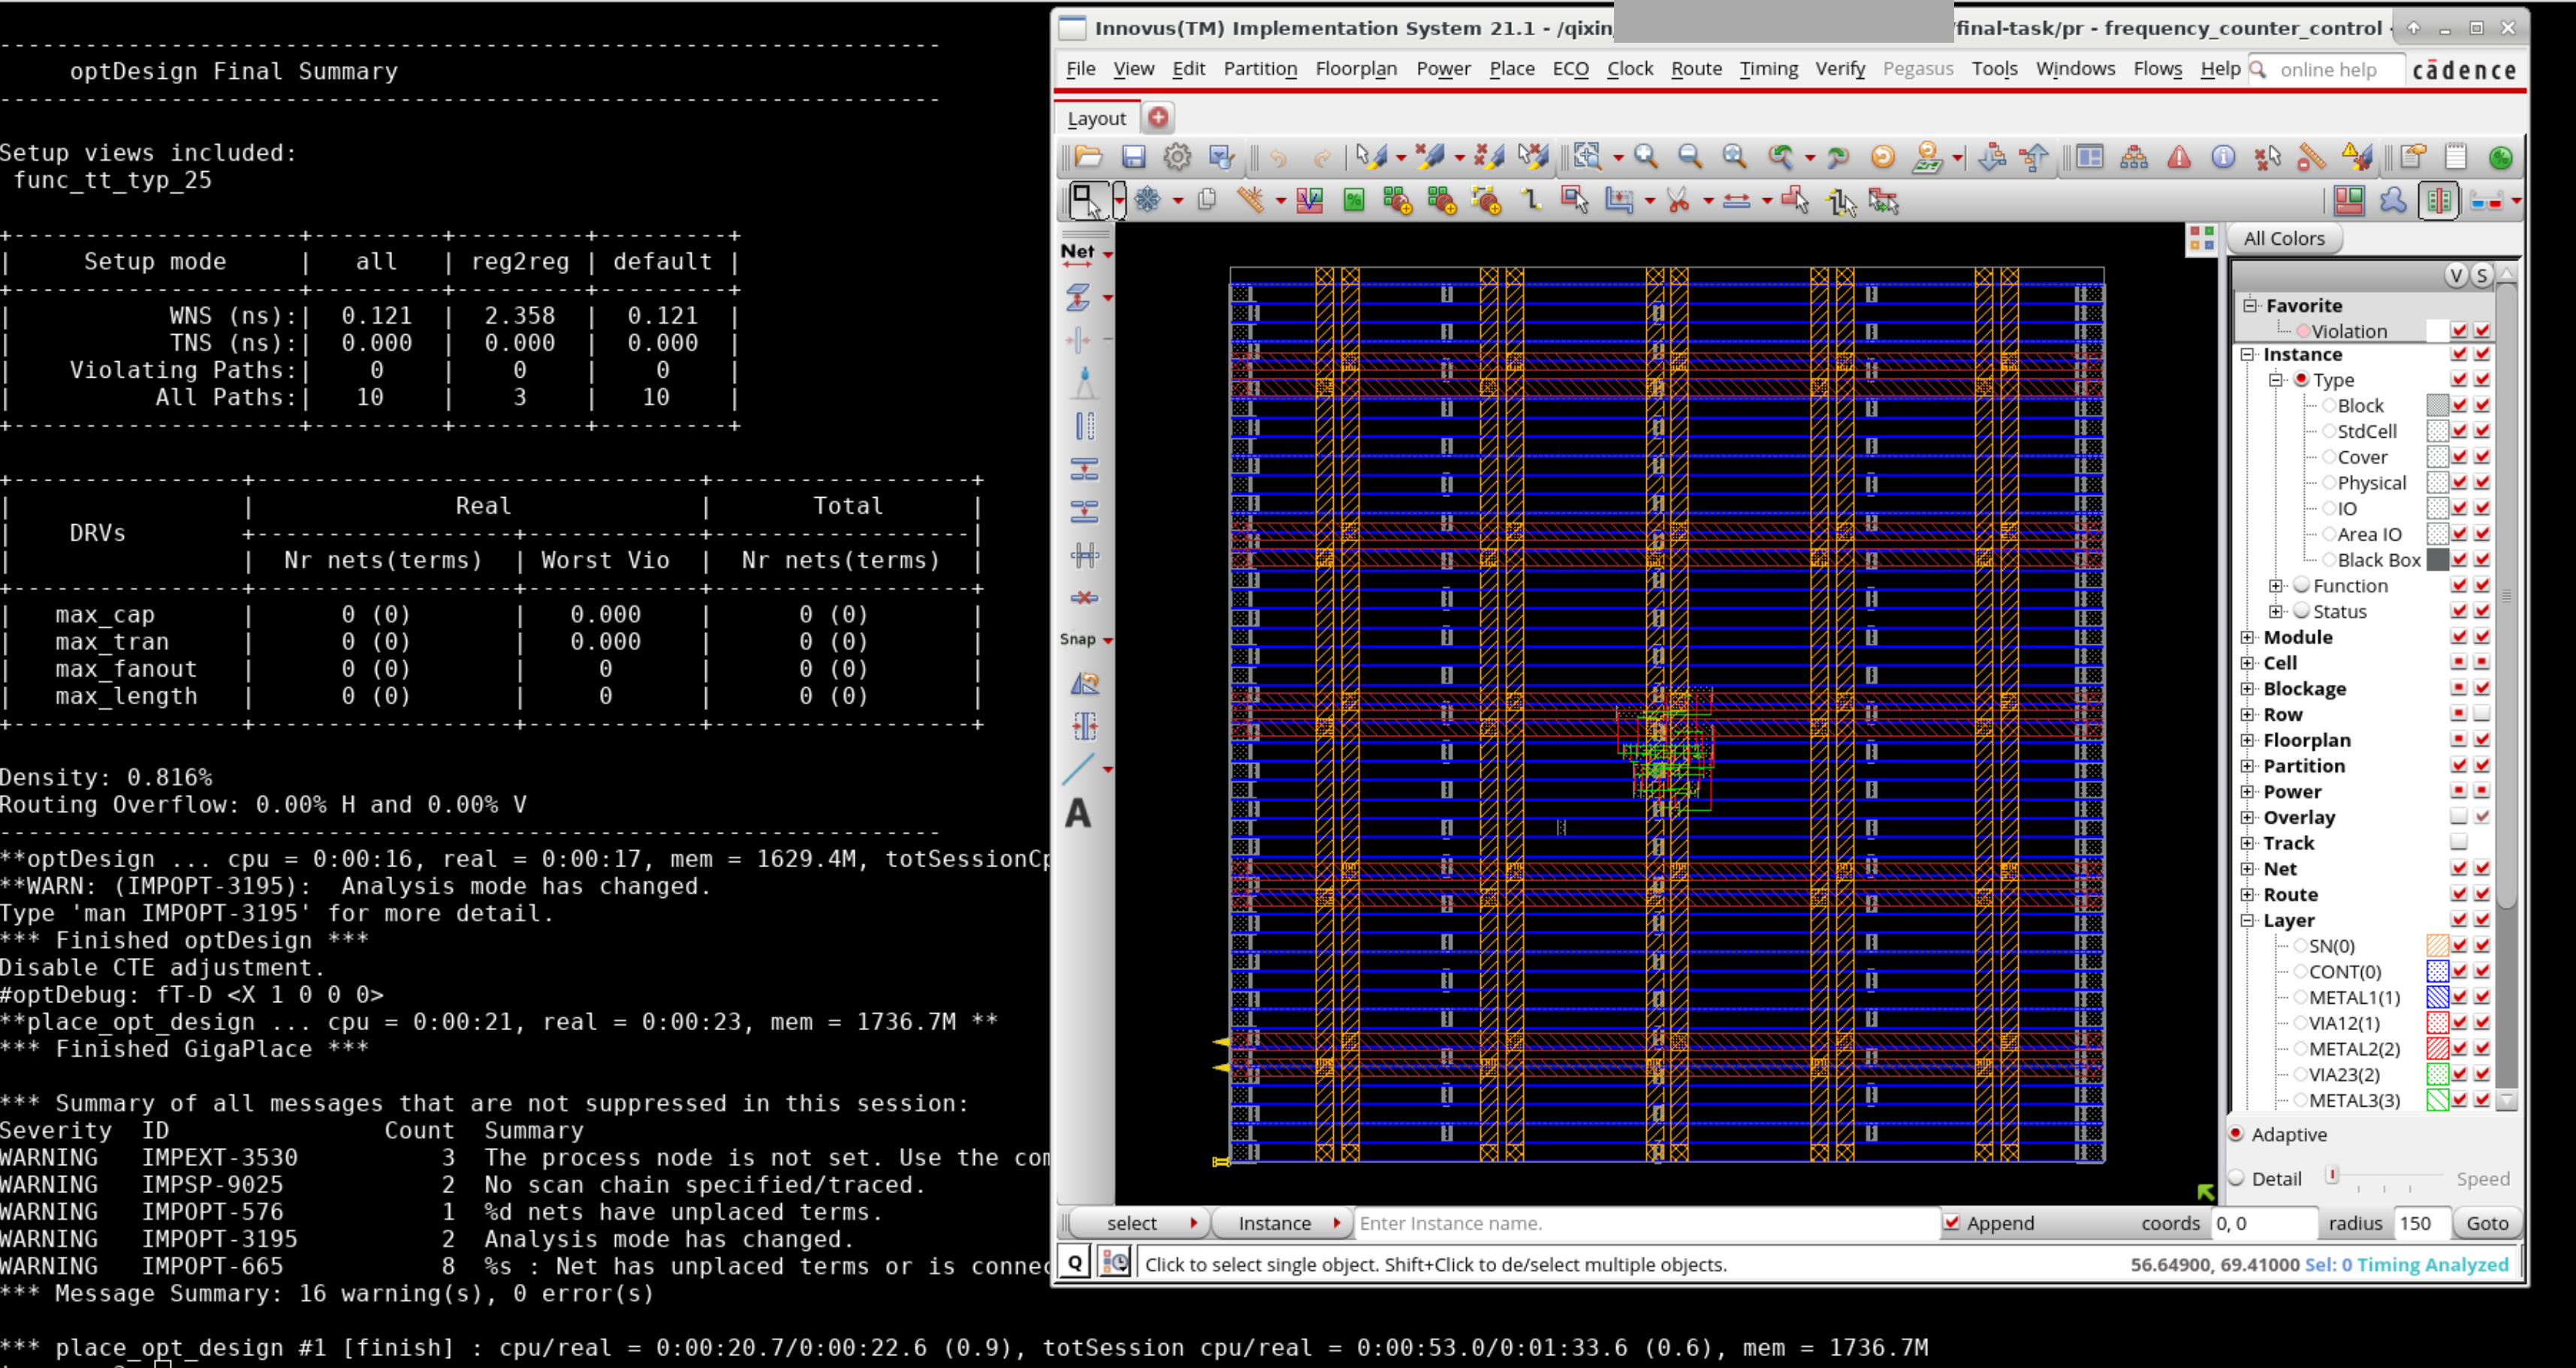
\includegraphics[width=0.8\textwidth]{images/final-task03-05.png}
    \caption{图6 布局布线}
\end{figure}

完成电源规划,运行 \texttt{run\_innovus\_step\_2\_powerplan.tcl}。

1) 定义全局电源规划

2) 添加 Power Stripe
    
3) 添加电源 follow pin

\begin{figure}[H]
    \centering
    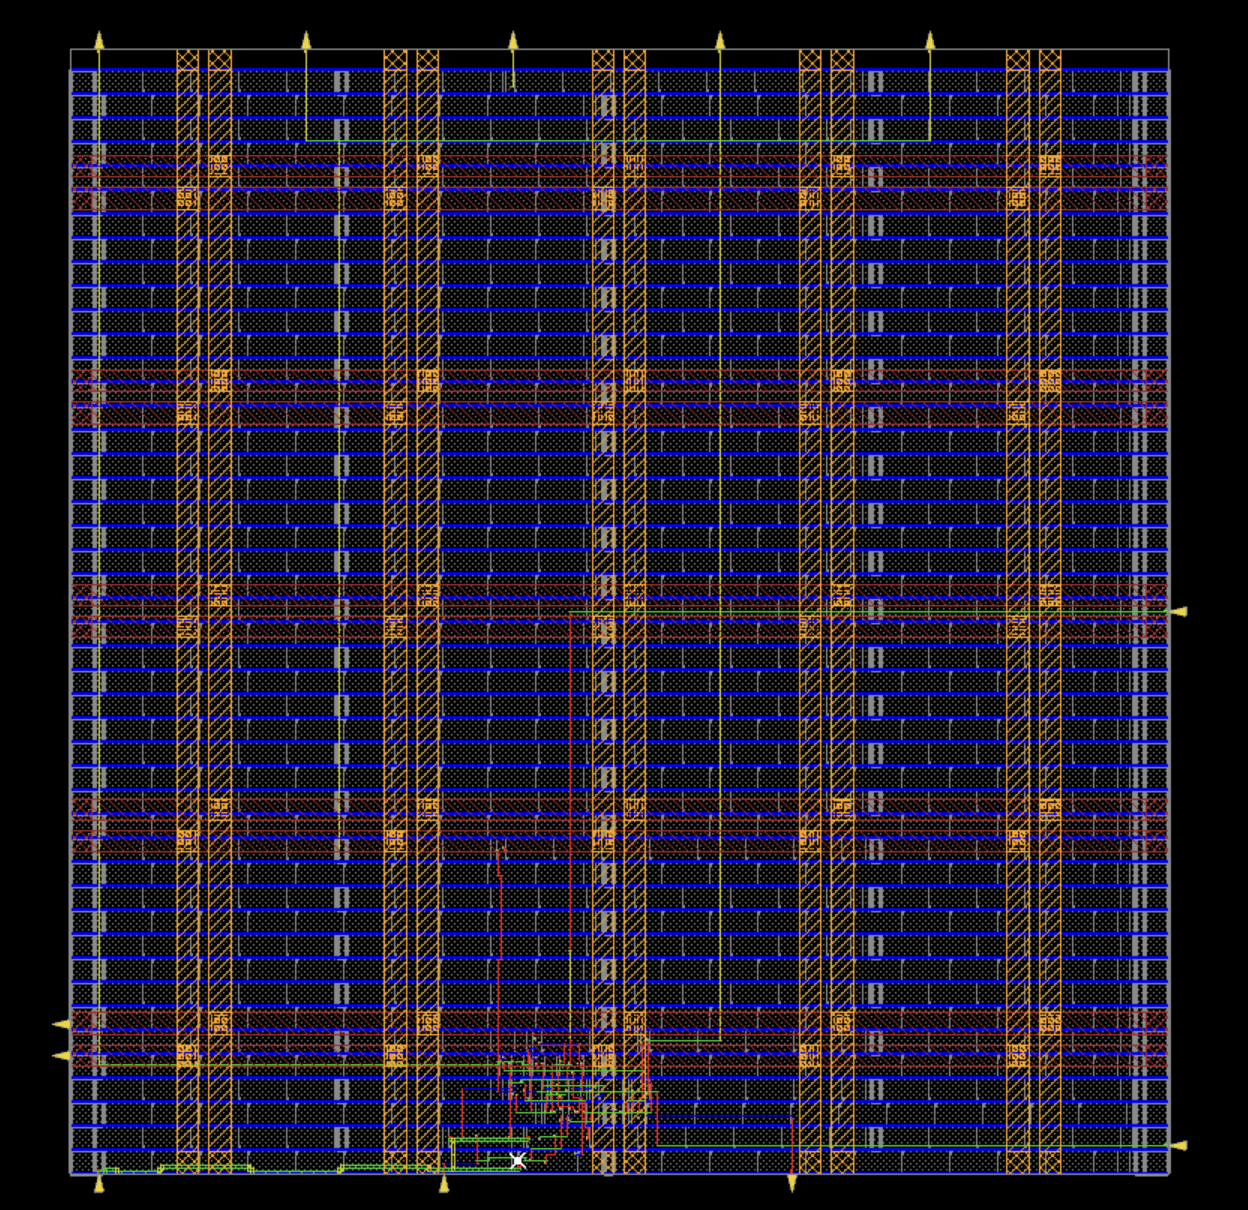
\includegraphics[width=0.8\textwidth]{images/final-task03-08.png}
    \caption{图7 电源规划}
\end{figure}

5. 保存数据

6. 完成plaecement

7. 检查place结果

8. CTS

9. 检查CTS结果

10. Route

\begin{figure}[H]
    \centering
    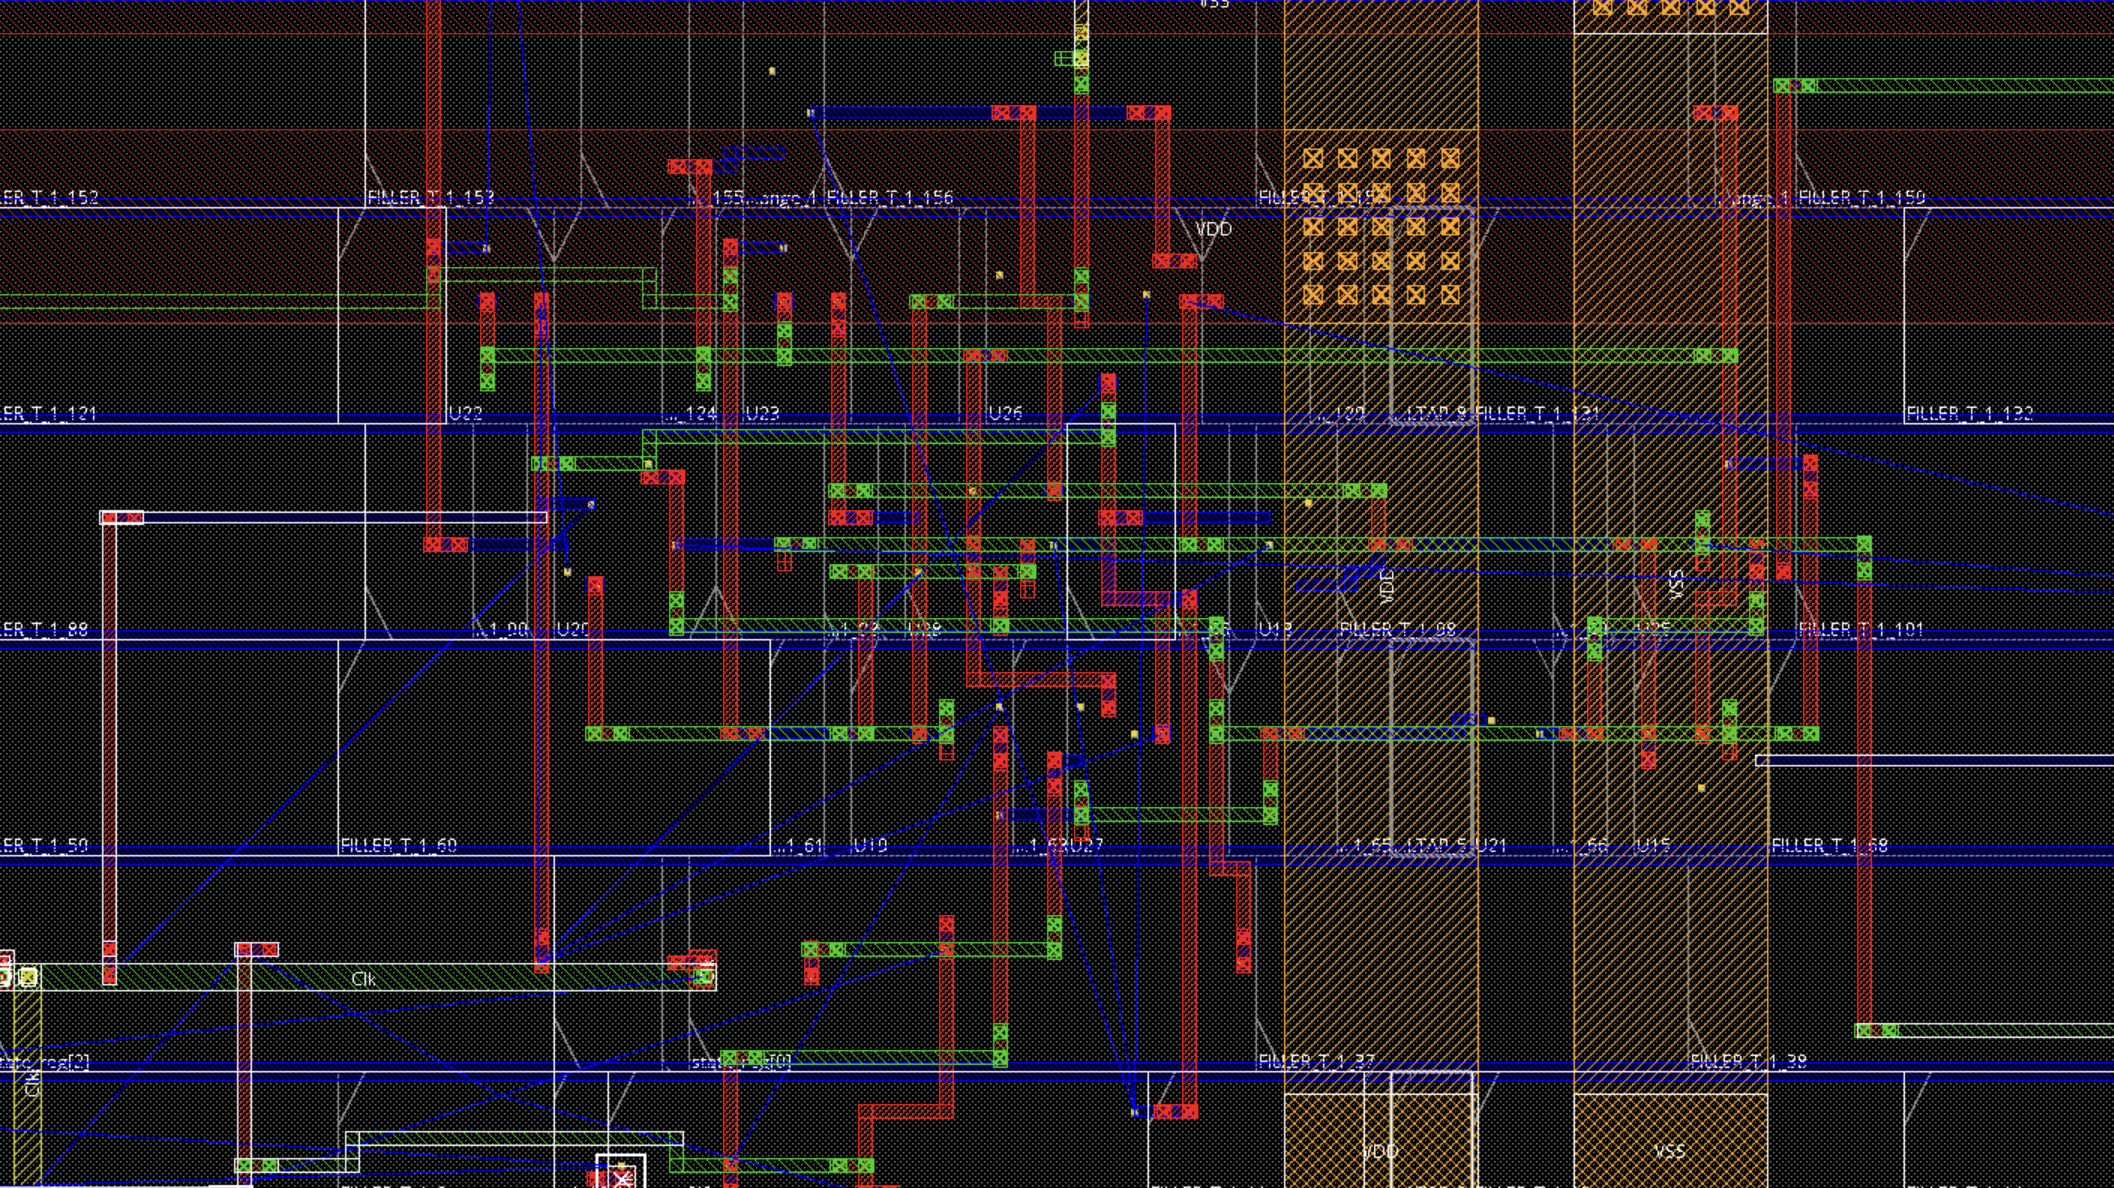
\includegraphics[width=0.8\textwidth]{images/final-task03-09.png}
    \caption{图8 布局布线}
\end{figure}

保存网表,命令:\texttt{saveNetlist route.v}
保存数据,命令:\texttt{saveDesign route.enc}
保存DEF,命令:\texttt{defOut -routing -withShield route.def}

\subsection{QRC 工具提取寄生参数}

使用 QRC 工具进行寄生参数的提取,使用 \texttt{qrc -cmd qrc.cmd},运行 qrc,如图所示:

QRC 提取运行完成:

\begin{figure}[H]
    \centering
    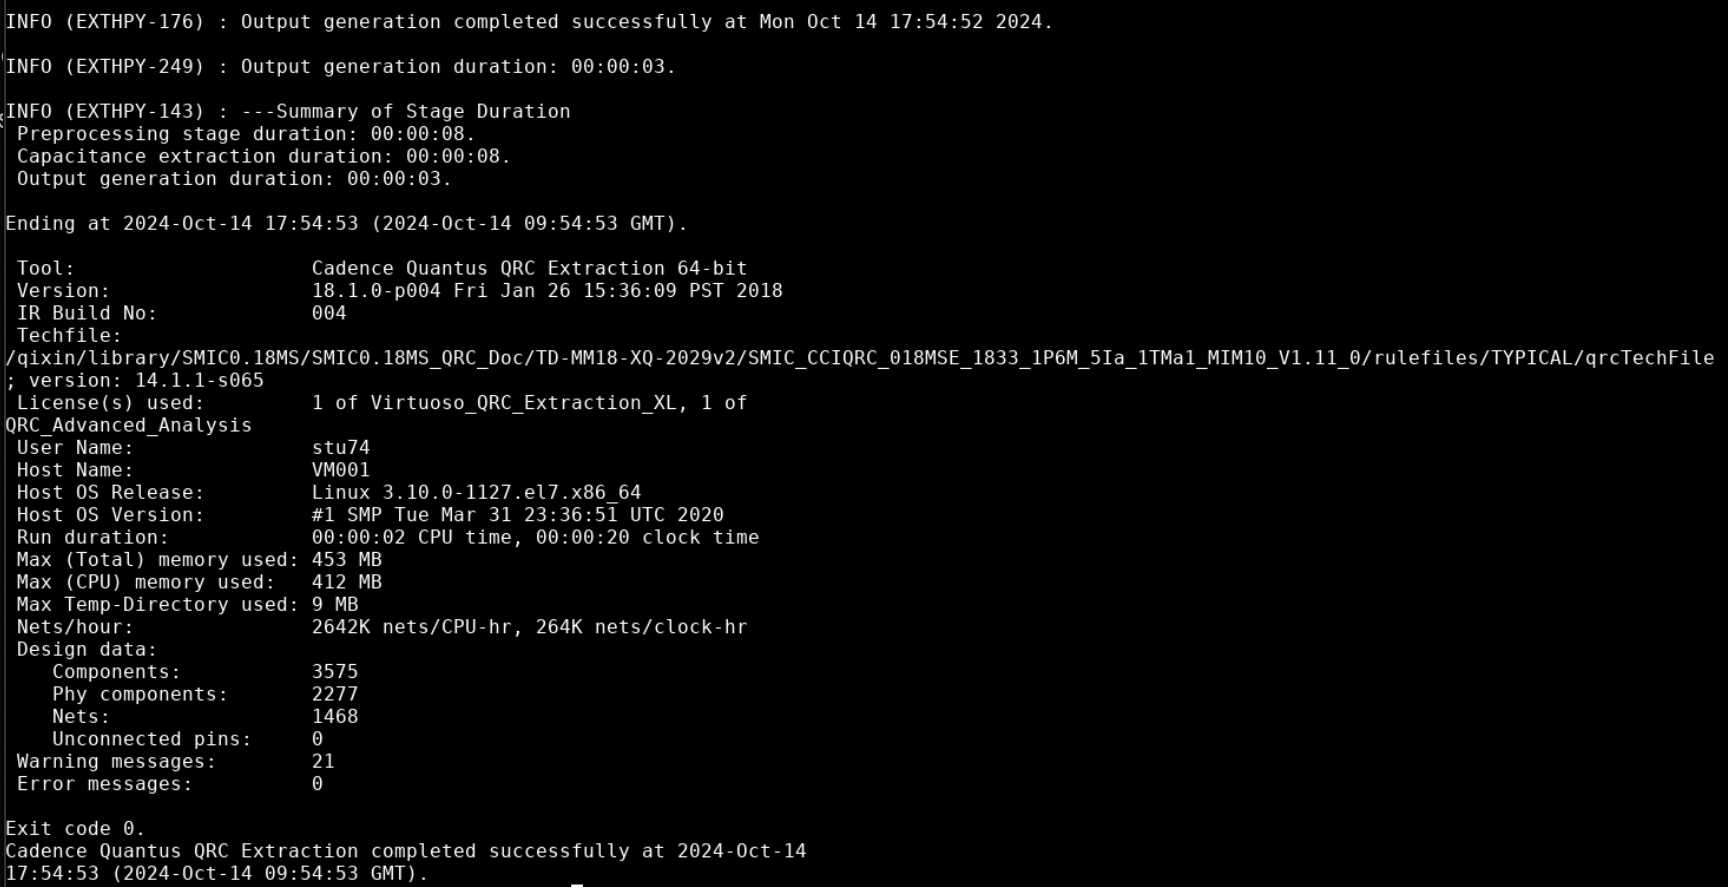
\includegraphics[width=0.8\textwidth]{images/final-task03-10.png}
    \caption{图9 QRC 提取结果}
\end{figure}

9. 进入到 \texttt{qrc\_test} 目录中,里面为提取出的寄生参数文件: \texttt{frequency\_counter\_control.spef}

\section{实验总结}

本任务通过Verilog编写频率计的控制部分,并使用状态机实现自动转换量程功能。完成仿真调试后,通过TCL脚本在Design Compiler中进行综合,确保时序裕度(slack)大于零,并生成.sdf文件用于后仿真。综合后的设计在Innovus工具中完成布局布线,通过时序检查和电源规划确保设计符合要求,最终生成网表和DEF文件作为输出结果。
